\documentclass{article}

\usepackage{listings}
\usepackage{hyphenat}
\usepackage{float}
\usepackage[T1]{fontenc}
\usepackage{hyperref,adjustbox}
\usepackage{graphicx}
\usepackage{pdfpages}
\usepackage[brazilian]{babel}
\usepackage{adjustbox}
\usepackage{multirow}
\usepackage{amssymb}
\usepackage{tabulary}
\usepackage{pifont}% http://ctan.org/pkg/pifont
\newcommand{\cmark}{\ding{51}}%
\newcommand{\xmark}{\ding{55}}%
\usepackage{tikz}
\usepackage{natbib}
\usepackage[T1]{fontenc}
\usepackage{enumitem}

\usepackage{titlesec}

\titleformat{\section}
  {\normalfont\Large\bfseries}{\thesection}{1em}{}[{\titlerule[0.8pt]}]


\title{Trabalho Prático - Parte 1 \\
\large Sistema de Recomendação para Moda}

\author{Heitor L. Werneck}
\begin{document}
\maketitle

\section{Introdução}
\subsection{Contextualização}
Um crescimento explosivo de quantidade de informação na Internet criou um desafio de sobrecarga de informações que impede o acesso a items de interesse. Esse fato aumentou a necessidade de sistemas de recomendação. Sistemas de recomendação são sistemas de filtragem de informações que lidam com o problema de sobrecarga de informações \cite{konstan2012recommender}, filtrando fragmentos de informações de uma grande quantidade de informações que é gerada dincamicamente por usuários utilizando um sistema de informação de acordo com seus interesses e prefêrencias sobre os items do sistema. Um sistema de recomendação tem a capacidade de prever se um determinado usuário preferiria um item ou não com base no histórico de consumo dos usuários.

Os sistemas de recomendação tem uma importância muito grande para grandes comércios, já que esses mesmo sistema tem a capacidade de influenciar em quantos items são comprados \cite{jannach2019measuring}. Os ganhos de lucro são observados em diversos comércios, como por exemplo: 35\% de aumento de vendas em um varejista de DVDs \cite{lee2014impact}; no eBay, \citeauthor{brovman2016optimizing} reportaram um aumento de 6\% em termos de lucro na implantação de um novo método de recomendação comparado ao modelo linear que estava sendo utilizado; diversos exemplos de sucesso são encontrados na literatura \cite{jannach2019measuring}.

A importância das vendas online no espaço da moda de luxo tem crescido em um ritmo acelerado nos últimos anos, já que os consumidores das indústrias tradicionais agora esperam fácil acesso a uma rede mundial de marcas e varejistas. Para ter sucesso neste cenário, é necessário fornecer uma experiência de compra de moda sob medida, personalizada e confiável. Os sistemas de recomendação desempenham um papel importante na jornada do usuário, permitindo que os clientes descubram produtos que atendem ao seu estilo, complementam suas escolhas ou os desafiam com novas ideias ousadas \cite{farfetchfashionrecommendationschallenge2021}.

Sistemas de recomendação de moda são tratados na literatura de diferentes prespectivas, como por exemplo: \citeauthor{wang2014intelligent} integra temas de moda e percepção humana sobre formas corporais personalizadas e conhecimento de designers profissionais; \cite{dong2020interactive} apresenta um sistema de recomendação de roupas que utiliza informações do formato 3D do corpo. No geral a literatura sobre recomendação no domínio de moda é escassa em relação a literatura de outros domínios, porém recentemente há um crescimento de interesse sobre domínio \cite{he2016ups,frejlichowski2016finding,wakita2015fashion,kang2017visually,zeng2013intelligent}. Existem trabalhos que propõem diversas técnicas de filtragem colaborativa, porém estes trabalhos divergem em mínimos pontos, como por exemplo no objetivo que varia muito de estudo para estudo, como por exemplo o estudo de \citeauthor{hu2015collaborative} que foca na criação de conjuntos de roupa (recomendação de um conjunto de itens). Porém, no geral há uma escassez de sistemas de recomendação que focam nesse domínio a partir de informações mais fundamentais da interação do usuário, as exceções são trabalhos como: \citeauthor{nguyen2014learning} que modela um método de learning to rank para recomendação personalizada de moda via feedback implicito (cliques, lista de desejos e compras), ainda é um método que pode ser generalizado para outros domínio e não há uma robusta avaliação quantitativa, comparando com métodos estado da arte, para comprovação de bons resultados.

\subsection{Objetivo}

Este trabalho propõe a criação de um sistema de recomendação competitivo para o domínio de moda que consiga explorar a larga gama de informações dos itens e usuários dadas pelo sistema de maneira eficaz e eficiênte, explorando padrões ainda não explorados no domínio. A base de dados de moda foi retirada de um desafio da FARFETCH para o ECML PKDD 2021, no qual o algoritmo criado aqui também tem o objetivo de ser utilizado na competição.

\section{Proposta}

A proposta deste trabalho consiste no desenvolvimento de um sistema de recomendação inovador para o domínio de roupas de moda, no qual específicamente será utilizado a base de dados de desafio da FARFETCH \footnote{\url{https://www.ffrecschallenge.com/ecmlpkdd2021/}}. Este trabalho espera contribuir com:

\begin{itemize}
   \item A modelagem de um sistema de recomendação competitivo para o cenário de recomendação de roupas de moda;
   \item Identificação dos padrões de consumo de usuários no domínio respectivo;
   \item Avaliação do modelo proposto comprovando sua utilidade;
   \item Submissão dos resultados para o desafio da FARFETCH no ECML PKDD 2021.
\end{itemize}

\section{Plano e Metodologia de Trabalho}

Para este projeto o cronograma e etapas de trabalho serão descritos a seguir, o modelo de processo em espiral será utilizado para realização das atividades.

\begin{enumerate}
   \item Estudo sobre o domínio e sistemas de recomendação: Primeira tarefa que consiste na obtenção de um conhecimento prévio sobre o domínio para capacitar a criação de soluções inovadoras. Essa tarefa também incluí o estudo e pesquisa de sistemas de recomendação próprios para o domínio, assim como genêricos e outros que exploram potênciais padrões de loja de moda.
   \item Obtenção da base de dados e preparação dos dados: Esta é a primeira tarefa em relação a implementação que será realizada e consiste simplesmente na coleta da base de dados do domínio específicado e a primeira preparação dos dados para serem pre-processados na etapa seguinte;
   \item Pré-processamento da base de dados: Esta etapa é onde haverá o pre-processamento da base, que inicialmente será somente para preparação dos dados para experimentação posterior, que será revisitada posteriormente a criação dos modelos de recomendação para aumentar a utilidade do recomendador;
   \item Propor e implementar métodos de recomendação: Nessa etapa o sistema de recomendação será elaborado e implementado, também sistemas de recomendação já existentes serão implementados, como por exemplo: Random (baseline); Popular; Item-kNN; User-kNN; SVD; NMF; SVD++ \cite{koren2008factorization}; NCF \cite{he2017neural} e outros. Assim como a composição desses métodos atráves de \textit{ensembles} pode ser explorada.
\begin{enumerate}[label*=\arabic*.]
   \item Implementação da métodologia de treinamento: Essa é uma etapa, que normalmente não seria destacada com seu proprio item, ficando implicito no item anterior, porém o treinamento e afinação de um modelo vem se mostrado extremamente importante, pois é um ponto na experimentação no qual diversos modelos se tornam não reprodutiveis em uma pequena mudança, sendo ela fundamental para bom funcionamento de um modelo (principalmente em um baseado em redes neurais) \cite{crane2018questionable,dacrema2019we}. Então, nesta etapa ocorrerá a criação e definição de métodologias para treinamento dos algoritmos, tanto para parâmetros quanto para hiperparâmetros, como por exemplo treinamento por minibatch, ou afinação de hiperparâmetros com k-fold cross-validation e entre outros;
\end{enumerate}
   \item Implementação da métodologia de avaliação e função objetivo: Nessa etapa a métodologia de avaliação e uma métrica objetivo do problema serão implementadas, que no caso será o \textit{Mean Reciprocal Rank} (MRR)) e seu ambiente para execução será definido para que posteriormente recomendadores possam ser avaliados;

   \item Execução dos recomendadores e análise dos resultados: Nesta etapa o sistema criado previamente será análisado frente a função objetivo do problema, assim como padrões e casos de sucesso obtidos pela solução criada para o problema, podendo ser por outras métricas que abordam a utilidade de diferentes maneiras, como por exemplo: NDCG, F1, Recall e outras.
   \item Escrita do artigo: Nesta etapa o trabalho será formalizado e a proposta será escrita no formato de artigo acadêmico, contendo: introdução, referêncial teorico, artigos relacionados, metodologia e conclusão.
\end{enumerate}
\subsection{Cronograma}

Abaixo, na tabela \ref{tbl:crono}, um cronograma estimado foi criado sobre a execução das atividades.
\begin{table}[!hbt]
\noindent\makebox[\textwidth]{
      \begin{tabular}{|l|c|c|c|c|}
         \hline
                                                                                    & \multicolumn{4}{c|}{Meses} \\\hline
         Atividade a ser realizada                                                  & 5                                   & 6      & 7      & 8 \\\hline
         1. Estudo sobre o domínio e sistemas de recomendação                       & \xmark                              & \xmark &        & \\\hline
         2. Obtenção da base de dados e preparação dos dados                        & \xmark                              &        &        & \\\hline
         3. Pré-processamento da base de dados                                      &                                     & \xmark &        & \\\hline
         4. Propor e implementar métodos de recomendação                            &                                     & \xmark & \xmark & \\\hline
         4.1. Implementação da métodologia de treinamento                           &                                     & \xmark & \xmark & \\\hline
         5. Implementação da métodologia de avaliação e função objetivo             &                                     &        & \xmark & \\\hline
         6. Execução dos recomendadores e análise dos resultados                    &                                     &        & \xmark & \\\hline
         7. Escrita do artigo                                                       &                                     &        & \xmark & \xmark \\\hline
\end{tabular}}
   \caption{Cronograma.}
   \label{tbl:crono}
\end{table}

\section{Problema}

O problema de recomendação foi definido por \citeauthor{burke2011recommender} como: Seja $U$ o conjunto de todos os usuários e seja $I$ o conjunto de todos os itens possíveis que podem ser recomendados, seja $\pi$ uma função de utilidade que mede a utilidade do item $i$ para o usuário $u$, ou seja, $\pi: U \times I \rightarrow R$, onde R é um conjunto totalmente ordenado, então para cada usuário $u$ queremos u item $i \in I$ que maximiza a utilidade do usuário.

Neste trabalho o problema será mais especificamente predizer qual produto que foi mostrado a um usuário levou a um clique, baseado nas interações que possuem rótulo de clique. Ou seja, os itens são subconjuntos de $I$ específicos para cada usuário, e no caso esse subconjunto tem cardinalidade 6.

Também o problema de sistemas de recomendação vem sendo estudado por muitos anos e é um problema no qual desafios para diversos domínios são conhecidos, no caso de moda desafios próprios do domínio ainda não são sistematicamente descritos pelo melhor do meu conhecimento. Porém a grande parte dos recomendadores sofrem por alguns problemas bem conhecidos, que são desafios na área, como por exemplo \cite{khusro2016recommender}: \textit{cold start problem}, no qual um novo usuário ou item entra no sistema; explicabilidade, que é geralmente encontrado a falta desse mesmo conceito em recomendadores baseados em redes neurais; \textit{grey sheep}, no qual um usuário não está de acordo com nenhum outro grupo (métodos de filtragem colaborativa normalmente sofrem desse problema); esparsidade, onde os usuários normalmente interagem em um sistema com um amplo catálogo de items e a distinção entre interações sobre items de usuários torna a matriz de interações esparsa, o que pode levar a recomendações com menos acurácia.


\section{Métodologia de avaliação}

A métodologia de avaliação deste trabalho inicialmente estará de acordo com a específicação dada no desafio da FARFETCH.

Nesse problema a tarefa de recomendação será a predição do próximo produto a ser consumido pelo usuário de uma lista de 6 produtos (que corresponde a uma requisição ou interação do usuário com o sistema). Essa tarefa tem como objetivo a maximização da utilidade para os usuários, que é definida como o \textit{Reciprocal Rank}.

Como dito anteriormente a utilidade do usuário será definida como o \textit{Reciprocal Rank}, e a utilidade média do recomendador será computada usando o \textit{Mean Reciprocal Rank} (MRR). O MRR é definido na equação \ref{eq:mrr}, onde $n$ são as impressões dos usuários sobre uma lista de items recomendados, e nessa equação dado a impressão $i$ o $rank_i$ é o rank da primeira predição correta.

\begin{equation}
   \label{eq:mrr}
   MRR = \frac{1}{|n|}\sum_{i=1}^{|n|}\frac{1}{rank_i}
\end{equation}

A base de testes é dada no desafio e consiste em amostras de 1 impressão para cada usuário, que podem estar no treino ou não, como será visto posteriormente na análise da base de dados.

\section{Base de Dados}

A base de dados que será utilizada foi provida pelo desafio da FARFETCH\footnote{\url{https://www.ffrecschallenge.com/ecmlpkdd2021/}}, no qual uma larga amostragem de impressões e eventos de clique no sistema de recomendação da FARFETCH foi feito durante um periodo de 2 meses. No qual, no total tem-se 5000000 eventos de recomendação, 450000 produtos e 230000 usuários unicos. A base de dados possui dados reais de interações de usuários com um sistema real na plataforma da FARFETCH, que porém são todos anonimizados (como por exemplo: usuário, produto, categórias, preços, marcas e etc). Além do contexto do usuário, os produtos também possuem atributos que o descreve. É importante notar que essa base possui diferentes amostras para fases definidas pelo desafio e neste trabalho será usado os dados da fase 1. Na fase 1 temos na verdade somente 4195182 eventos, 219035 usuários e 443150 produtos, que é uma base com esparsidade de 99.996749\%.

Uma coisa que será possível observar nas subseções a seguir é que grande parte dos atributos são categóricos. Os atributos anonimizados são representados por padrão como uma cadeia de 64 caracteres, que podem, posteriormente na fase de pre-processamento serem transformados em outros atributos e também podem ser selecionados.

\subsection{Análise das Interações dos Usuários}

Os atributos dos objetos das interações são descritos a seguir na tabela \ref{tbl:inter} (Obs: os valores únicos foram obtidos pelo conjunto de dados de treino):

\begin{table}[!hbt]
\noindent\makebox[\textwidth]{
      \begin{tabular}{|c|c|c|c|p{7cm}|}
         \hline
      Atributo             & Escala  & Cardinalidade & \#Valores únicos & Descrição \\\hline\hline
      query\_id            & Nominal & Discreta      & 584665           & identificador único da impressão de recomendação \\\hline
      user\_id             & Nominal & Discreta      & 208393           & identificador único do usuário\\\hline
      session\_id          & Nominal & Discreta      & 317426           & identificador único da sessão de navegação\\\hline
      product\_id          & Nominal & Discreta      & 408263           & identificador único do produto\\\hline
      page\_type           & Nominal & Discreta      & 5                & tipo de página em que a recomendação foi mostrada\\\hline
      previous\_page\_type & Nominal & Discreta      & 23               & tipo de página em que o usuário navegou antes de ver a recomendação\\\hline
      device\_category     & Nominal & Discreta      & 3                & tipo do dispositivo\\\hline
      device\_platform     & Nominal & Discreta      & 2                & plataforma do dispositivo\\\hline
      user\_tier           & Ordinal & Discreta      & 6                & identificador do nível de usuário no programa de recompensa FARFETCH\\\hline
      user\_country        & Nominal & Discreta      & 196              & identificador do país de onde o usuário está navegando\\\hline
      context\_type*       & Nominal & Discreta      & 4                & uma string que identifica o tipo de contexto. Os valores possíveis são "designer\_id", "category\_id" e "product\_id" (correspondendo às páginas de lista de designer, páginas de lista de categoria e páginas de produto, respectivamente) \\\hline
      context\_value*      & Nominal & Discreta      & 187906           & o ID correspondente da entidade fornecida em context\_type\\\hline
      is\_click            & Ordinal & Binária       & 2                & 1 se o produto foi clicado, 0 se não\\\hline
      product\_price       & Razão   & Continua      & 1757598          & preço normalizado do produto no momento dado\\\hline
      week                 & Ordinal & Discreta      & 8                & número normalizado da semana em que o evento aconteceu\\\hline
      week\_day            & Ordinal & Discreta      & 7                & dia da semana em que o evento aconteceu\\\hline
\end{tabular}}
   \caption{Descrição geral dos atributos das interações. ''*'' indica atributo que pode conter múltiplos valores.}
   \label{tbl:inter}
\end{table}

Na base obtida, somente o atributo context\_type possui valores faltantes, que corresponde a 4\% dos objetos. Ou seja, no geral essa base de dados não sofre de muitas irregularidades. No geral não há um alto número de diferentes categorizações para as interações do usuário, diferentemente dos produtos como será visto posteriormente. O número baixo de atribuições para o atributo 'week' evidência um outro fato da base já mencionado anteriormente, que é uma base de um curto periodo temporal que pode limitar a utilização e exploração dos padrões temporais de longo prazo ou de temporadas, fazendo atributos temporais não parecerem tão interessantes a primeiro instante, porém padrões temporais de curto período ainda podem existir.

\subsection{Análise dos Produtos}

Os atributos dos objetos de produtos são descritos a seguir na tabela \ref{tbl:products}:

\begin{table}[!hbt]
\noindent\makebox[\textwidth]{
      \begin{tabular}{|c|c|c|c|p{7cm}|}
         \hline
         Atributo            & Escala  & Cardinalidade & \#Valores únicos & Descrição \\\hline\hline
         product\_id         & Nominal & Discreta      & 443150           & identificador do produto\\\hline
         gender              & Nominal & Discreta    & 4                & genêro do produto\\\hline
         main\_colour        & Nominal & Discreta      & 17               & a cor principal do produto\\\hline
         second\_colour      & Nominal & Discreta      & 22               & a segunda cor mais predominante do produto\\\hline
         season              & Nominal & Discreta      & 7                & temporada da moda\\\hline
         collection          & Nominal & Discreta      & 9                & identificador da coleção de moda\\\hline
         category\_id\_l1    & Nominal & Discreta      & 43               & primeiro nível da árvore de categorias de produtos\\\hline
         category\_id\_l2    & Nominal & Discreta      & 394              & segundo nível da árvore de categorias de produtos\\\hline
         category\_id\_l3    & Nominal & Discreta      & 583              & terceiro nível da árvore de categorias de produtos\\\hline
         brand\_id           & Nominal & Discreta      & 3399             & identificador da marca do produto\\\hline
         season\_year        & Nominal & Discreta      & 20               & ano da temporada da moda\\\hline
         start\_online\_date & Razão   & Contínua      & 2150             & número de dias online em relação a uma data de referência predefinida\\\hline
         attribute\_values*  & Nominal & Discreta      & 859              & atributos do produto, como informações adicionais sobre o tipo de produto e padrões\\\hline
         material\_values*   & Nominal & Discreta      & 129              & composição do material do produto\\\hline
   \end{tabular}

}
   \caption{Descrição geral dos atributos dos produtos. ''*'' indica atributo que pode conter múltiplos valores.}
   \label{tbl:products}
\end{table}

Não existe nenhum dado faltante nesse conjunto de dados. Pela tabela podemos ver a quantidade de valores únicos para esse conjunto de dados em cada um de seus atributos, primeiro é possível notar de maneira comparativa que muito mais categorias existem para os produtos, do que para os usuários, que é o esperado, pois normalmente os items são cadastrados por um administrador que deseja maxima efetividade e completude na descrição de seus produtos. Sobre o ponto de vista de mineração de dados, uma ampla gama de atributos pode abrir possibilidade para encontrar diferentes e diversos padrões no sistema, que podem ser valiosos, que porém podem atrapalhar se a amostragem de treinamento for pequena.

\subsection{Análise Geral e Básica}

Dado toda essa meta-análise da base, será mostrado nessa seção mais análises simples sobre os dados e comportamentos superficiais dos mesmos, só para dar uma ideia do comportamento da base nessa proposta. Esse é só uma amostragem de todas análises feitas, pois seria inviável colocar todas formalizadas aqui.

Um dos primeiros pontos a se observar é o comportamento de consumo de items pelos usuários. O gráfico abaixo mostra a taxa de consumo dos items, é possível observar que, assim como a maioria dos domínios de recomendação, possui uma cauda longa entre usuários e catálogo de itens.

\begin{figure}[ht]
    \centering
    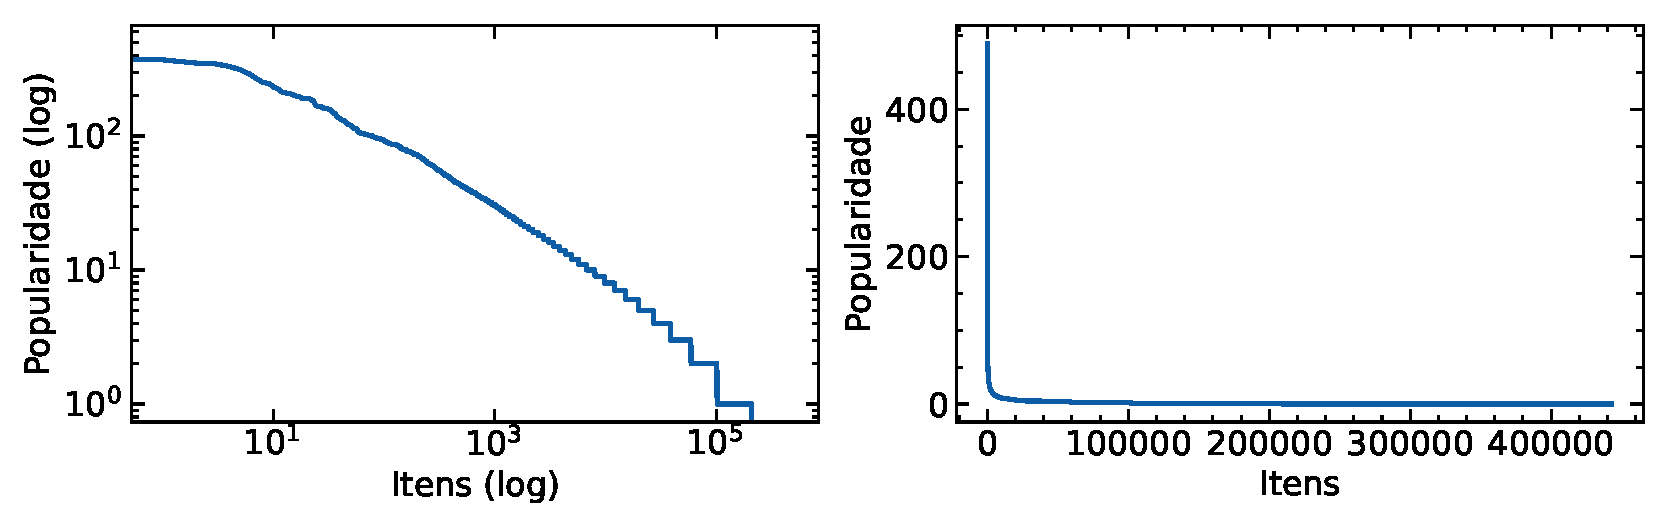
\includegraphics[width=1.00\textwidth]{items_pop.eps}
    \caption{Popularidade dos itens.}
    \label{fig:users}
\end{figure}

Também usuários nesse domínio de exibição de produtos para cliques podem recorrentemente clicar nos mesmos itens, como pode-se ver na tabela \ref{tbl:productuser}, porém a probabilidade é baixa como é possível observar na tabela abaixo que apresenta as porcentagens de frequências de clique de usuários em produtos, ou seja, nesse caso 96.8\% das interações entre usuário e produto tiveram somente 1 clique.

\begin{table}[!hbt]
\begin{center}
\begin{tabular}{|c|c|}
\hline
Quantidade de cliques &   Porcentagem de pares usuário-produto \\\hline
1  &  96.888511\% \\\hline
2  &   2.728706\% \\\hline
3  &   0.293456\% \\\hline
4  &   0.058175\% \\\hline
5  &   0.018416\% \\\hline
6  &   0.006712\% \\\hline
7  &   0.002754\% \\\hline
8  &   0.001377\% \\\hline
9  &   0.000516\% \\\hline
10 &   0.001205\% \\\hline
11 &   0.000172\% \\\hline
\end{tabular}
\end{center}
\caption{Distribuição de frequência de cliques em produtos por usuários}
  \label{tbl:productuser}
\end{table}

Também um outro ponto observado sobre a base de dados foi a presença de usuários e items \textit{cold start} no teste, isto é, a presença de usuários é de 9\% e items de 7\%. Parte significativa do teste são esses casos, o que mostra a necessidade de técnicas que tratam este problema para atingir um bom resultado. Também mensurar os ganhos sobre esse grupo de usuários é interessante.

\section{Resultados Preliminares}

Atualmente diversas proposta de recomendadores foram testadas como benchmark inicial, sem um treinamento e afinação de parâmetros robusto. Entre elas temos:

\begin{enumerate}
  \item NeuMF: Que é um método baseado em redes neurais, que funde a fatorização generalizada de matrizes por meio de redes neurais com camadas de multilayer perceptron. Uma ilustração do modelo é apresentada abaixo:

\begin{figure}[h]
    \centering
    \includegraphics[width=0.90\textwidth]{neumf.png}
    \caption{NeuMF.}
  \label{fig:neumf}
\end{figure}

  \item Popular: Popular é um modelo tradicional de baseline de sistemas de recomendação, esse método irá rankear os itens de acordo com o mais popular. A popularidade foi definida nesse trabalho como o número de diferentes usuários que clicaram no item.
  \item SVD (Singular Value Decomposition): O SVD é um método de fatorização de matrizes que é utilizado em sistemas de recomendação para filtragem colaborativa. 
  \item BilinearNet: É um baseline simples de aprendizado de embeddings com redes neurais, que não faz uso de nenhuma camada e aprende as representações dos usuários e itens.
  \item Random: Um modelo simples, para definir o lower bound do problema, que recomenda itens de maneira aleátoria.
  \item SVD++: É um método que minimiza uma função objetivo, que inclui um viés geral e outros 2 para os usuários e os itens, utilizando Stochastic Gradient Descent (SGD) assim como regularização com L2.
  \item Item-kNN: Método que mede a correlação dos itens e depois usa grupos desses itens para identificar o conjunto de itens a ser recomendado.
  \item User-kNN: Método que diferentemente do Item-kNN, ao invés de medir a similaridade entre itens, mede a similaridade entre usuários para após isso obter os itens que devem ser recomendados.
\end{enumerate}

Esses algoritmos e outros que não tiveram bons resultados foram executados, a tabela abaixo apresenta o MRR de cada um desses métodos:


\begin{table}[!hbt]
\noindent\makebox[\textwidth]{
      \begin{tabular}{|c|c|}
         \hline
       Métodos     & MRR \\\hline
       NeuMF       & 0.4315\\\hline
       Popular & 0.4213\\\hline
       SVD         & 0.4142\\\hline
       BilinearNet & 0.4139\\\hline
       Random      & 0.4119\\\hline
       SVD++       & 0.3873\\\hline
       Item-kNN    & Overflow de memória \\\hline
       User-kNN    & Overflow de memória\\\hline
\end{tabular}}
   \caption{Resultados de MRR.}
   \label{tbl:mrr}
\end{table}

Esses resultados ainda não são definitivos, problemas podem ter sido feitos nessa etapa do trabalho, que é muito inicial, porém podemos ver que o aleátorio não se diferencia muito dos outros algoritmos. O que se destaca é o NeuMF com bons resultados, em segundo o Popular que conseguiu resultados consideraveis comparado aos outros algoritmos, demonstrando que nessa base os outros modelos com um pouco mais de complexidade talvez não sejam suficientes. O SVD++ que é um baseline normalmente competitivo teve resultados ruins, demonstrando a não trivialidade do domínio.

Os métodos apresentam baixa diferenciação de resultados em relação ao aleatório, demonstrando que os métodos atuais ainda não estão bons, assim como o problema é difícil.

Os usuários e itens cold start podem ter grande impacto nesses resultados, o que necessita de maior investigação em trabalhos futuros.

Outras investigações de inserção de contexto em métodos foram óvaliadas, porém ainda não foi possível obter um resultado satisfatório.

\section{Conclusão}

Com esté trabalho inicial foi possível definir formalmente o problema assim como demonstrar a importância do seu desenvolvimento. O desafio a ser solucionado foi formalizado e a metodologia de avaliação já foi possível ser definida. Assim como um entedimento melhor sobre a base dados a ser utilizada foi dado.

Já foi possível observar alguns resultados preliminares, que parecem evidenciar a baixa capacidade de aprendizado dos métodos. Trabalhos futuros também precisam ser realizados, como por exemplo: avaliar melhor e aprimorar a metodologia de treinamento dos algoritmos; inserir contexto dos usuários e dos items na recomendação personalizada; adicionar mecanismos para recomendação de itens para usuários cold start; explorar ideias de seleção de features ou redução de dimensionalidade após a criação de métodos que suportam features externas; reduzir o problema de overfitting nos modelos de redes neurais; modelagem do problema de predição como uma tarefa de predizer o próximo item na sequência.

\bibliographystyle{plainnat}
\bibliography{doc.bib}
\end{document}
